\documentclass[conference]{ieeeconf}

\usepackage[utf8]{inputenc}
\usepackage[T1]{fontenc}
\usepackage{listings}
\usepackage{biblatex}
\usepackage{graphicx}

\title{\LARGE \bf
Prevent overcrowding in exhibitions using FogFlow to distribute people}

\author{\IEEEauthorblockN{Lorenzo Siega Battel}
\IEEEauthorblockA{Politecnico di Milano}
\IEEEauthorblockA{lorenzo.siega@mail.polimi.it}}

\addbibresource{main.bib}

\begin{document}
\maketitle
\thispagestyle{empty}
\pagestyle{empty}

\begin{abstract}

The organizers of an exhibition with several booths are trying to avoid overcrowded booths so visitors could be distributed smoothly and enjoy the exhibition. They mount sensors at each booth so to know the number of people currently at each booth. Each booth has an electrical board which, based on the information from other booths their distance, suggests visitors the closest booth to visit next in a way that the population is smoothly distributed. The overall number of visitors of each booth is reported to the cloud for information aggregation to be queried for the crowded time of the day.

\end{abstract}

\section{Introduction}
During an exhibition people can stop in front of a booth and create congestion. By providing them informations about the next more suitable booth to visit, we can distribute them more efficiently and so avoid overcrowding.\\
People at each booth are counted using cameras or some other types of sensors and then an algorithm suggest, for each both, a booth to visit by displaying it on an "electrical board".\\
In this document we will address the problem by leaving the choice of the sensor and the algorithm to the final people who finally implement the system.\\
During the development of such a system two main problems will have to be addressed:
\begin{itemize}
    \item Required analysis effort: As we have to analyze a stream of data from a large number of sensors, we can't compute it on a centralized component.
    \item Algorithm: Algorithm works on the entire set of booths and triggering it on each update received from a booth, as FaaS computing does, will generate an high computation and data load.
\end{itemize}{}
FogFlow can address to both problems, by filling these gaps:
\begin{quote}
    \begin{enumerate}
        \item[G2] Function triggering: from per event to per selected entities: In existing serverless computing frameworks, functions are invoked per event with limited execution time and memory size. This is not suitable for data-intensive IoT services.[...]
        \item[G3] Function execution: from data $\rightarrow$ code or code $\rightarrow$ data to code $\leftrightarrow$ data: Existing serverless computing frameworks separate data management from the function execution environment, always moving data into the execution environment for function execution (data to code pattern). On the other hand, existing fog computing frameworks such as Azure IoT Edge move cloud functions to the data located at the edges.[...]
        \item[G4] Function composition: from event-oriented or edge-oriented to data-centric: 
        In existing serverless computing frameworks such as OpenWhisk, service developers need to customize a series of event triggers and rules to link multiple functions together. Existing fog computing frameworks allow service developers to link functions at each edge by manually configuring the topic-based data routing path between them.[...]
    \end{enumerate}{}
    \cite{cheng2019fog}
\end{quote}

\section{Context producers and context consumers}
In FogFlow, as it is a data-centric framework, our first goal is to produce data, process it and then utilize that data to make decisions or let others do that.\\
In this document we will refer at data as context. In fact, in FogFlow, data is handled as a context and not as a single entity, so multiple instances of a single entity can create a context.
For example you can think of multiple sensors that count people who are entering in a building, a single sensor can produce a context called “Ingoing at entrance 2-A” while all the sensors placed at the entrances of a building can produce a context called “People flow in building 2”.
FogFlow can handle this different types of context producing different other context updates based on where they will be "deployed". For example it can reduce the flow at a single entrance or cut it when a building is becoming full of people.
\subsection{Context producer aka the sensor}
We cannot know \textit{a priori} the pyhisical structure of an exhibition so we do not provide any constraint on the type of the sensor.
Sensor's data will be processed on site and then sent to the nearest broker adoptingits  NGSI10 APIs.

\subsection{Context consumer aka the electronic board}
As for the sensor we cannot know how informations will be displayed so an intermediate device is needed to receive data from FogFlow and then show it.\\
It will expose an HTTP server which will be used by the broker to send context updates.
\begin{figure}[ht]
    \centering
    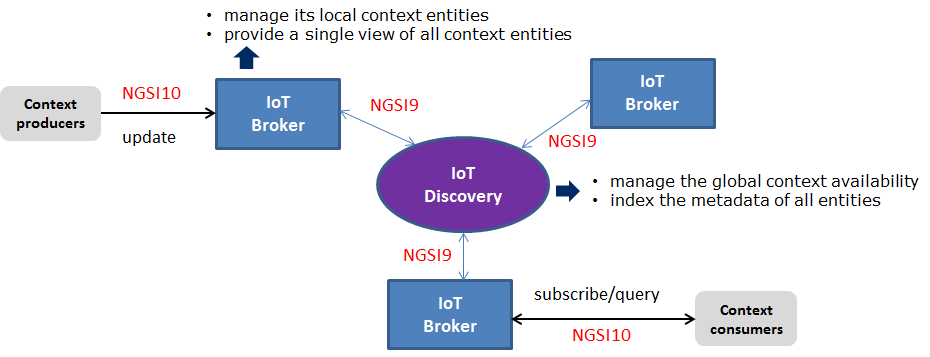
\includegraphics[width=0.5\textwidth]{Images/distributed-brokers.png}
    \caption{Context prod/cons topology}
\end{figure}{}

\section{Operator and Fog Function}
An operator contains the Fog Function code and must be in the form of a docker image and available on Docker Hub. 
FogFlow enables serverless edge computing, meaning that developers can define and submit a so-called fog function and then the rest will be done by FogFlow automatically, including:
\begin{itemize}
    \item Triggering the submitted fog function when its input data are available
    \item Deciding how many instances to be created on workers according to its defined granularity
    \item Deciding where to deploy the created instances
\end{itemize}{}
The instances in the above text refer to the task instances which run a processing logic within them and this processing logic is given by the operator.
\begin{figure}[ht]
    \centering
    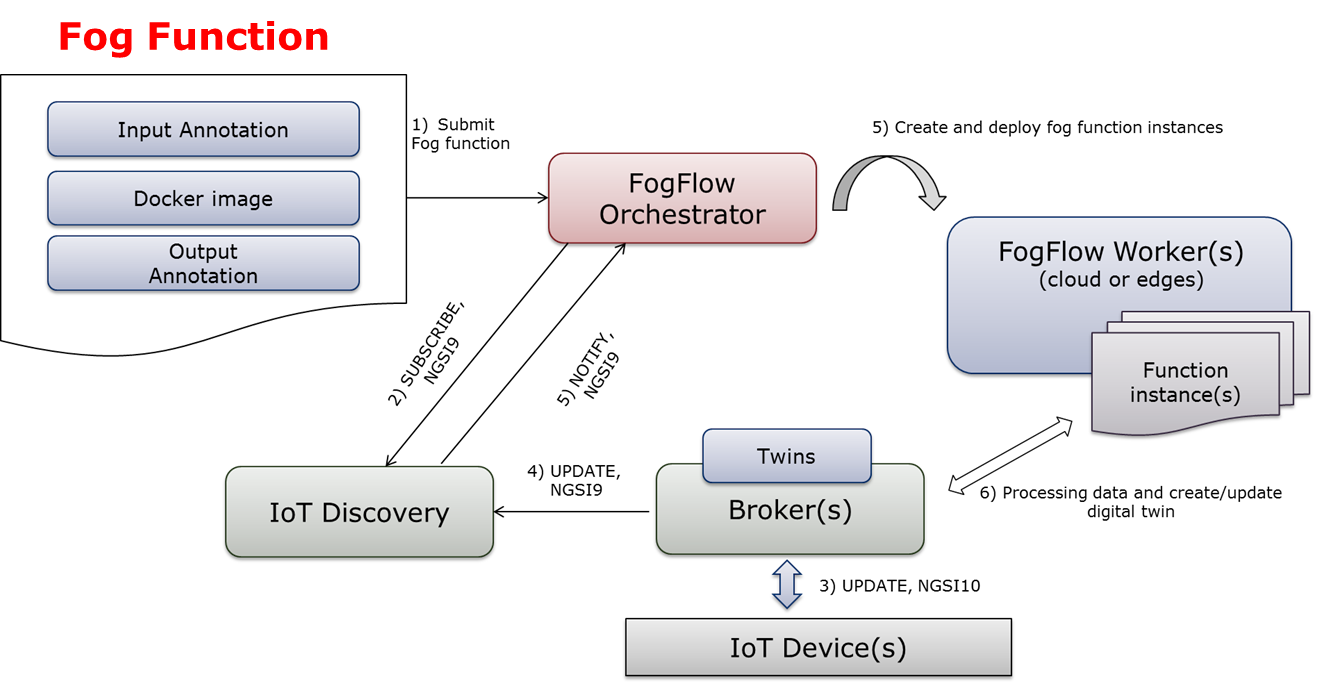
\includegraphics[width=0.5\textwidth]{Images/function-orchestration.png}
    \caption{FogFlow and Fog Functions}
\end{figure}{}

\section{Data visualization and querying}
To better provide insights on how people move through the exposition and to allow the organizers to perform queries on the data, a scraping tool is mandatory.
Prometheus is the best choice for two reasons:
\begin{itemize}
    \item It allows users to perform queries on its data directly and not by using other tools
    \item It's widely supported by data visualization tools like Grafana
\end{itemize}{}
Perhaps the broker must be modified to expose a web service that matches the syntax accepted by Prometheus.
Please notice that from now on we will see three values for each counter (count, male and female). These values are chosen by the developer (the broker exposes the values uploaded by the context producers) and so they are not fixed.
Below an example of this syntax and in the next page the Go code developed.
\begin{lstlisting}
PeopleCounter_1{name="count"} 56
PeopleCounter_1{name="male"} 37
PeopleCounter_1{name="female"} 19
PeopleCounter_10{name="count"} 45
PeopleCounter_10{name="male"} 37
PeopleCounter_10{name="female"} 8
PeopleCounter_20{name="count"} 17
PeopleCounter_20{name="male"} 14
PeopleCounter_20{name="female"} 3
\end{lstlisting}{}

\subsection{Querying}
To perform queries we must use a language called PromQL that lets the user select and aggregate time series data in real time.
In the following examples, of PromQL, we assume there is a counter for each booth.
\begin{itemize}
    \item Affluence for each booth:
    \begin{lstlisting}[breaklines=true]
{__name__=~"PeopleCounter_.*", name="count"}
    \end{lstlisting}{}
    \item Total affluence, per gender:
    \begin{lstlisting}[breaklines=true]
sum({__name__=~"PeopleCounter_.*", name="male"})
sum({__name__=~"PeopleCounter_.*", name="female"})
    \end{lstlisting}{}
    \item Affluence at a specific booth:
    \begin{lstlisting}[breaklines=true]
PeopleCounter_10{name="count"}
    \end{lstlisting}{}
\end{itemize}{}

\subsection{Visualization}
To visualize data generated by the sensor, in some different graphs, and to provide an immediate point of view in a dashboard, Grafana is the best tool to use.
In fact it allows us to use directly the data produced by the PromQL queries for build some interesting graphs.
\begin{figure}[ht]
    \centering
    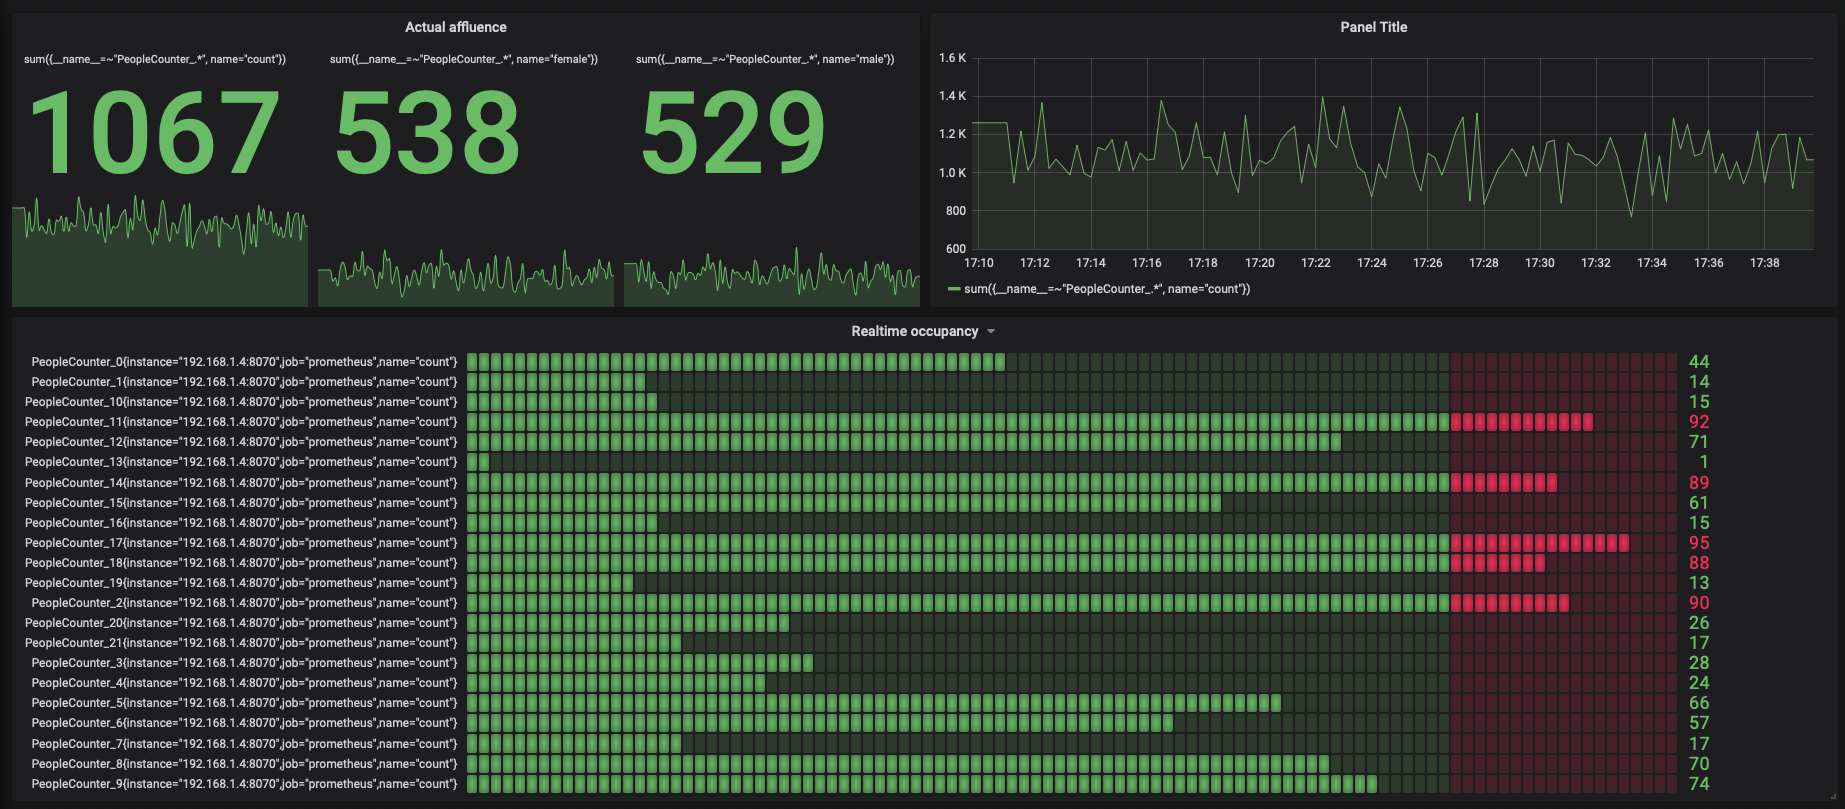
\includegraphics[width=0.5\textwidth]{Images/dashboard.png}
    \caption{A dashboard created using the queries in the example above}
\end{figure}{}

\printbibliography

\onecolumn
\begin{lstlisting}[language=go, breaklines=true]
func (apisrv *RestApiSrv) getEntitiesProm(w rest.ResponseWriter, r *rest.Request) {
  for _, entity := range apisrv.broker.getEntities() {
    for _, attribute := range entity.Attributes {
      val, err := strconv.ParseFloat(fmt.Sprintf("%v", attribute.Value), 64)
      if err == nil {
        w.(http.ResponseWriter).Write([]byte(fmt.Sprintf("%s{name=\"%s\"} %v\n", strings.ReplaceAll(entity.Entity.ID, ".", "_"), attribute.Name, val)))
      }
    }
  }
}

func (apisrv *RestApiSrv) getEntityProm(w rest.ResponseWriter, r *rest.Request) {
  var eid = r.PathParam("eid")

  entity := apisrv.broker.getEntity(eid)
  if entity == nil {
    w.WriteHeader(404)
  } else {
    for _, attribute := range apisrv.broker.getEntity(eid).Attributes {
      val, err := strconv.ParseFloat(fmt.Sprintf("%v", attribute.Value), 64)
      if err == nil {
        w.(http.ResponseWriter).Write([]byte(fmt.Sprintf("%s{name=\"%s\"} %v\n", strings.ReplaceAll(entity.Entity.ID, ".", "_"), attribute.Name, val)))
      }
    }
  }
}

func (apisrv *RestApiSrv) getAttributeProm(w rest.ResponseWriter, r *rest.Request) {
  var eid = r.PathParam("eid")
  var attrname = r.PathParam("attr")

  attribute := apisrv.broker.getAttribute(eid, attrname)
  if attribute == nil {
    w.WriteHeader(404)
  } else {
    val, err := strconv.ParseFloat(fmt.Sprintf("%v", attribute.Value), 64)
    if err == nil {
      w.(http.ResponseWriter).Write([]byte(fmt.Sprintf("%s{name=\"%s\"} %v\n", strings.ReplaceAll(eid, ".", "_"), attribute.Name, val)))
    }
  }
}
\end{lstlisting}{}
\end{document}